\documentclass[25pt,a0paper]{tikzposter}
 %\usepackage[absolute,overlay]{textpos}
 \usepackage[english]{babel}
\usepackage[utf8]{inputenc}
\usepackage[T1]{fontenc}
%\usepackage{url}
\usepackage{multicol}
\usepackage{amsfonts,amssymb,amsmath,amsthm}
\tikzposterlatexaffectionproofoff
\usepackage{color}
\usepackage{bm} % pour le gras
\usepackage{blindtext}
\usepackage{comment}

\graphicspath{{figures/}}

\usepackage[backend=bibtex]{biblatex}

\addbibresource{abbr,denise.bib} 

% algorithm
\usepackage{etoolbox}
\AtBeginEnvironment{algorithm}{%
  \setlength{\columnwidth}{\linewidth}%
}
\usepackage{algorithm}
\usepackage{algorithmic}

 
 %% definitions des commandes
 
\newcommand{\vct}[1]{\bm{#1}} %vecteurs
\newcommand{\mtx}[1]{\bm{#1}} %matrices

\DeclareMathOperator*{\diag}{diag}
\DeclareMathOperator*{\argmax}{arg\,max} % Operators for argmin and argmax (_{} under the operator)
\DeclareMathOperator*{\argmin}{arg\,min}

\newcommand{\vbar}[1]{#1_{\overline{v}}} % similar to x_v, but with overline over v
\def\Phivbar{\vbar{\Phi}} % previous command applied to \Phi
\def\xvbar{\vbar{x}} % previous command applied to x
\def\C{\mathbb{C}} % ensembles des nombres complexes
\def\R{\mathbb{R}} % ensembles des nombres réelles


\title{From audio inpainting to phase retrieval}
\author{Louis Bahrman, Marina Krémé, Paul Magron, Antoine Deleforge}
\institute{Université de Lorraine, CNRS, Inria, Loria, F-54000 Nancy, France}

\makeatletter
\newcommand\insertlogoi[2][]{\def\@insertlogoi{\includegraphics[#1]{#2}}}
\newcommand\insertlogoii[2][]{\def\@insertlogoii{\includegraphics[#1]{#2}}}
\newlength\LogoSep
\setlength\LogoSep{0pt}

\insertlogoi[width=9cm]{inr_logo_rouge_cmjn}
\insertlogoii[width=9.3cm]{logo_anr}


\renewcommand\maketitle[1][]{  % #1 keys
    \normalsize
    \setkeys{title}{#1}
    % Title dummy to get title height
    \node[transparent,inner sep=\TP@titleinnersep, line width=\TP@titlelinewidth, anchor=north, minimum width=\TP@visibletextwidth-2\TP@titleinnersep]
        (TP@title) at ($(0, 0.5\textheight-\TP@titletotopverticalspace)$) {\parbox{\TP@titlewidth-2\TP@titleinnersep}{\TP@maketitle}};
    \draw let \p1 = ($(TP@title.north)-(TP@title.south)$) in node {
        \setlength{\TP@titleheight}{\y1}
        \setlength{\titleheight}{\y1}
        \global\TP@titleheight=\TP@titleheight
        \global\titleheight=\titleheight
    };

    % Compute title position
    \setlength{\titleposleft}{-0.5\titlewidth}
    \setlength{\titleposright}{\titleposleft+\titlewidth}
    \setlength{\titlepostop}{0.5\textheight-\TP@titletotopverticalspace}
    \setlength{\titleposbottom}{\titlepostop-\titleheight}

    % Title style (background)
    \TP@titlestyle

    % Title node
    \node[inner sep=\TP@titleinnersep, line width=\TP@titlelinewidth, anchor=north, minimum width=\TP@visibletextwidth-2\TP@titleinnersep]
        at (0,0.5\textheight-\TP@titletotopverticalspace)
        (title)
        {\parbox{\TP@titlewidth-2\TP@titleinnersep}{\TP@maketitle}};

    \node[inner sep=0pt,anchor=west] 
      at ([xshift=-\LogoSep]title.west)
      {\@insertlogoi};

    \node[inner sep=0pt,anchor=east] 
      at ([xshift=\LogoSep]title.east)
      {\@insertlogoii};

    % Settings for blocks
    \normalsize
    \setlength{\TP@blocktop}{\titleposbottom-\TP@titletoblockverticalspace}
}
\makeatother
 
\usetheme{Simple}
\begin{document}
  \maketitle
 \begin{columns}
 \column{.5} % premiere colonne
\block{OVERVIEW}{
 \begin{tikzfigure}
   \label{fig:example}
    \centering
    \includegraphics[width=\linewidth]{figures/example.png}\\ % == \linewidth,non ? oui si tu veux, si c'est pas trop grand . 
    %Sinon on set heigth en ca genere des erreurs ils me semble ?
% Ok, j'ai effectivement jamais set une height en cm
 \textbf{Goal}: reconstructing the missing samples $\vct{x}_{\bar{v}} \in \mathbb{R}^{d}$ of a signal $\vct{x}^{\star} \in \mathbb{R}^{L}$ from its discrete Fourier transform (DFT) magnitudes $\vct{b} \in \mathbb{R}_+^L$ and some known samples $\vct{x}_{v}=\vct{y} \in \mathbb{R}^{L-d}$.
\end{tikzfigure}

\hspace{0.1cm}
\innerblock{Contributions}{
\begin{itemize}
        \item A problem formulation that highlights the connection to phase retrieval
        \item A Gerchberg-Saxton (GS)-like alternating projection algorithm 
        \item Investigation of a suitable initialization
    \end{itemize}
}
}
%\begin{itemize}
    %\item \textbf{Goal}: reconstructing missing audio $\vct{x}_{\bar{v}}$(blue curve)  from magnitudes of discrete Fourier transform and some samples  $\vct{x}_{v}$  (orange curve)
   % \item \textbf{Current results}:
    %\begin{itemize}
    %    \item Proposed problem formulation
        %\item Connection with phase retrieval
        %\item Investigation of a suitable initialization for the implementation of an alternating projection algorithm 
   % \end{itemize}
    
%\end{itemize}


\block {PROPOSED METHOD}{
%$\triangleright$  \textbf{Notation}:
    % \begin{itemize}
        %\item Let $\vct{x} \in \mathbb{R}^{L} $ be a time domain signal for which only $v$ samples are observed.
        %\item Let $\bar{v}$ the set of the missing indices of $\vct{x}$ and $d$ the cardinal of $\bar{v}$
        %\item Let $\mtx{\Phi} \in \C^{L\times L}$ be a Fourier matrix
        % \item Known part of the signal $\vct{x}$:  $\vct{y} \in \mathbb{R}^{L-d}$ %and $d$ the cardinal of $\bar{v}$ the unknown part 
        %of $\vct{x}$ and $\vct{x}_{\bar{v}}$ its missing part.
        % \item Observations of the DFT magnitudes: $\vct{b} \in \mathbb{R}^{L}_{+}$
    % \end{itemize}
    % \hspace{0.1cm}
    % \innerblock{Audio inpainting formulation}{
    % \begin{align*}
    %  %\label{eqn:audioInpaintingForm}
    %     \text{find} \; {\vct{x}_{\bar{v}}} \in \mathbb{R}^{d} \; \text{s.t.}
    %     \begin{cases}
    %         |\mtx{\Phi} \vct{x} |&= \vct{b} \\
    %         \vct{x}_{v}&= \vct{y}
    %     \end{cases}
    % \end{align*}
    % }
    %$\triangleright$ \textbf{Problem \eqref{eqn:audioInpaintingForm} study}: rely on existing results in the context of phase retrieval\cite{Gerchberg1972,Waldspurger2015,Candes2015b,Candes2011}
%\vspace{1.5cm}
%\coloredbox[fgcolor=gray]{\centering \Large \textbf{Connection to phase retrieval}}
%\vspace{1.5cm}

\textbf{Problem setting}
\vspace{1 cm}
%
\begin{equation*}
   \vct{x}^{\ast} =  \underset{\vct{x} \in \R^{L}}{\text{argmin}}\,\|  |\mtx{\Phi} \vct{x} | -\vct{b}\|^{2} \quad \text{s.t.} \quad \vct{x}_{v}= \vct{y}
\end{equation*}
%
where $\mtx{\Phi} \in \mathbb{C}^{L \times L}$ is the DFT matrix.

\vspace{1cm}
\textbf{Connection to phase retrieval}
\vspace{1 cm}
\begin{itemize}
    \item Consider the auxiliary phase variable: $\vct{u} \in \C^{L}$ with $|\vct{u}| = 1$.
    %= phase (\mtx{\Phi} \vct{x}) = \displaystyle \frac{\mtx{\Phi} \vct{x}}{|\mtx{\Phi} \vct{x}|} \in \C^{L}$.
    \item The inpainting problem can be rewritten as ~\cite{Waldspurger2015}:
\begin{equation*}
    \vct{x}^{\ast},\vct{u}^{\ast} =  \underset{\vct{x} \in \R^{L}, \vct{u} \in \C^{L}}{\text{argmin}}\,\|\mtx{\Phi} \vct{x}- \diag(\vct{b})  \vct{u}\|^{2}  \quad \text{s.t.}  \quad  |\vct{u}| =1 \quad \text{and}  \quad \vct{x}_{v}= \vct{y}
\end{equation*}
 \vspace{0.5em}
    \item Decompose $\mtx{\Phi}$ and $\vct{x}$ as: 
    %$\mtx{\Phi}  =[\mtx{\Phi}_{v},\mtx{\Phi}_{\bar{v}}]$ 
\begin{center}
\vspace{-3em}
    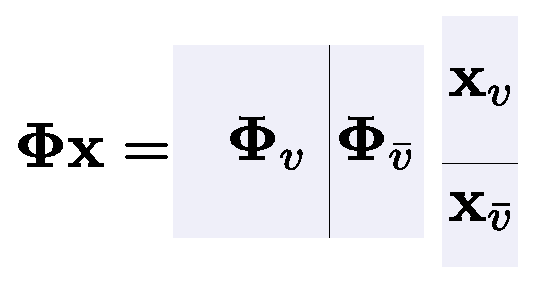
\includegraphics[scale=0.9]{phi_x_bar.eps}
\end{center}
%We assume $\mtx{\Phi} =[\mtx{\Phi}_{v},\mtx{\Phi}_{\bar{v}}]$ (where $\mtx{\Phi}_{v} =\mtx{\Phi}_{:,v}$ ) and $\vct{x} = [\vct{x}_{v};  \vct{x}_{\bar{v}}]$ where $[.,.]$ (resp. $[.;.]$) denote horizontal and (resp. vertical) concatenations. 
    \item Since $\mtx{\Phi}$ is a unitary matrix (with Hermitian transpose $\mtx{\Phi}^{\mathsf{H}}$), the problem rewrites:
\begin{equation*}
   \vct{x}_{\bar{v}}^{\ast},\vct{u}^{\ast} =  \underset{\vct{x}_{\bar{v}} \in \R^{d}, \vct{u} \in \C^{L}}{\text{argmin}}\,\|\vct{y}- \mtx{\Phi}_{v}^{\mathsf{H}}\diag(\vct{b}) \vct{u}\|^{2} +  \|\vct{x}_{\bar{v}}- \mtx{\Phi}_{\bar{v}}^{\mathsf{H}}\diag(\vct{b}) \vct{u}\|^{2} \quad \text{s.t.}  \quad  |\vct{u}| = 1%phase (\mtx{\Phi} \vct{x})
\end{equation*}
% \begin{equation*}
%   \vct{x}_{\bar{v}}^{\ast},\vct{u}^{\ast} =  \underset{\vct{x}_{v}= \vct{y}, \; \vct{u} = phase (\mtx{\Phi} \vct{x})}{\text{argmin}}\,\|\vct{x}_{v}- \mtx{\Phi}_{v}^{\mathsf{H}}\diag(\vct{b}) \vct{u}\|^{2} +  \|\vct{x}_{\bar{v}}- \mtx{\Phi}_{\bar{v}}^{\mathsf{H}}\diag(\vct{b}) \vct{u}\|^{2},
% \end{equation*}
\end{itemize}

\vspace{1cm}
\textbf{Alternating projections algorithm}
\vspace{1 cm}
\begin{itemize}
    \item Given $\vct{u}$, the solution is $\vct{x}_{\bar{v}} =\mtx{\Phi}_{\bar{v}}^{\mathsf{H}}\diag(\vct{b}) \vct{u}$.
    \item To find $\vct{u}$, we consider:
    \begin{equation*}
   \vct{u}^{\ast} =  \underset{\vct{u} \in \C^{L}}{\text{argmin}}\, \|\vct{x}- \mtx{\Phi}^{\mathsf{H}}\diag(\vct{b}) \vct{u}\|^{2}   \quad \text{s.t.}  \quad  |\vct{u}| = 1 
\end{equation*}
which leads to $\vct{u} = phase (\mtx{\Phi} \vct{x}) = \displaystyle \frac{\mtx{\Phi} \vct{x}}{|\mtx{\Phi} \vct{x}|}$.
\end{itemize}

%\begin{itemize}
%    \item Initialize $\vct{x} = \vct{x}^{(0)}$ with $\vct{x}^{(0)}_{v}= \vct{y}$
%    \item Repeat until convergence:
%\end{itemize}

\vspace{2em}
\begin{center}
    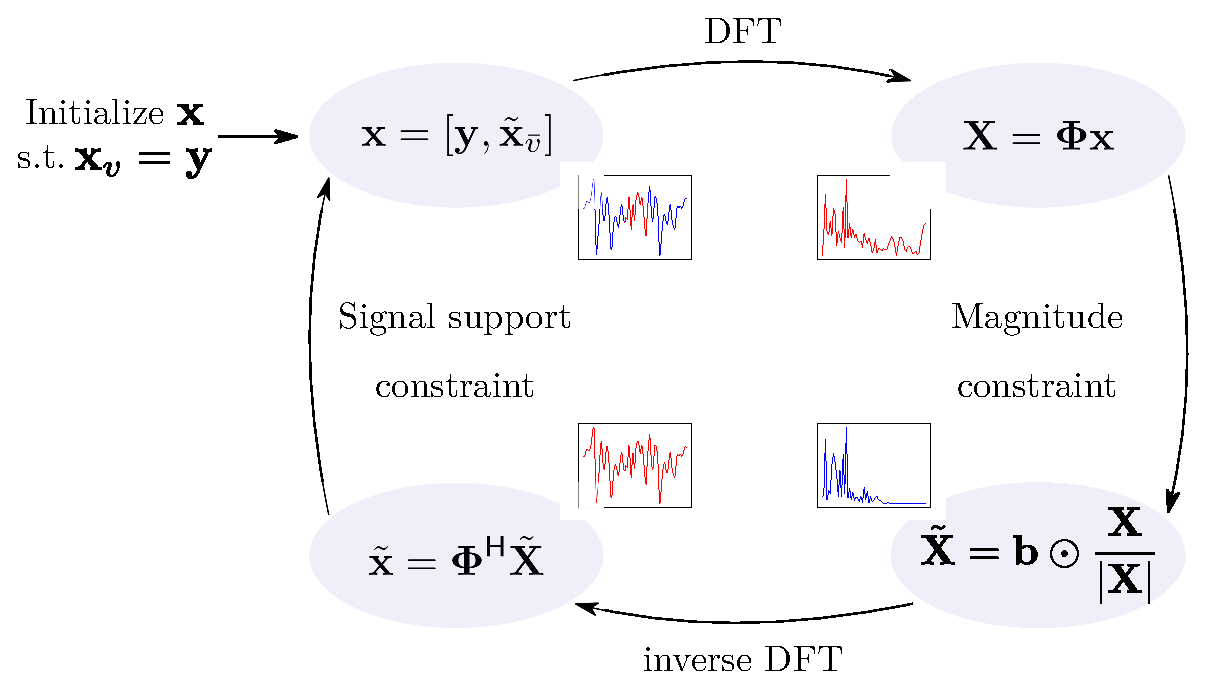
\includegraphics[scale=1.8]{inpainting_alt_projsvg.eps}
\end{center}
}


%\block{AUDIO INPAINTING like GS}{
% \begin{algorithm}[H]
%     \caption{Audio inpainting like GS algorithm}
%     \label{algoAlternatedMinimization}
%     \begin{algorithmic}
%     \REQUIRE
%     $\begin{cases}
%         \vct{b} \in \R^{L}_{+}:  \text{observations}\; n_\text{iter}  : \text{number of iterations}\; \text{and} \; \varepsilon: \text{threshold}\\
%         \vct{x}_{v}: \text{known signal}\\
%         \mtx{\Phi}: \text{Fourier matrix}
%     \end{cases}$
%     \vspace{0.5cm}
% \ENSURE{$\vct{x}_{\bar{v}}^{\ast}$ predicted missing signal}
%   \STATE Initialization: 
%   ${\vct{x}^{0}_{\bar{v}} \leftarrow \text{spectral initialization from} \; \mtx{Y} =\Phi_{\bar{v}}^{\mathsf{H}}\diag(\vct{b})\Phi_{\bar{v}}}$ \; \text{and} \;{$\vct{x}^{0} \leftarrow [\vct{x}^{0}_{v}, \vct{x}_{\bar{v}}] $}
%   \STATE i=0
%   \WHILE{$i<n_\text{iter} \;\text{and} \; \||\mtx{\Phi} \vct{x} | -\vct{b}\|^{2} > \varepsilon $}
%  \STATE  $\vct{u} \leftarrow phase (\mtx{\Phi} \vct{x}^{(i)})$
%  \STATE $\vct{x}_{\bar{v}}^{(i)} \leftarrow \mtx{\Phi}_{\bar{v}}^{\mathsf{H}}\diag(\vct{b}) \vct{u}$
%  \STATE $\vct{x}^{(i)} \leftarrow [\vct{x}^{0}_{v}, \vct{x}_{\bar{v}}^{(i)}] $
%  \STATE i= i+1
%     \ENDWHILE
%   \end{algorithmic}
%       \end{algorithm}
%}



\column{.5} % deuxiem colonne
\block{PRELIMINARY NUMERICAL SIMULATIONS}{

\textbf{Data}:
\begin{itemize}
    \item $100$ speech excerpts from the Librispeech dataset, sampled at $16$ kHz.
    \item Signal length: $L \in  \{128,512, 2048\}$ samples.
    \item Fraction of deleted signal: from $ 5 \%$ to $50 \%$.
\end{itemize}
%All experiments have been conducted using extracts from the Librispeech dataset  \cite{librispeech}. The total length of the signal varied in $\{128,512, 2048\}$ samples, at 16kHz. The fraction of deleted signal $\frac{d}{L}$ varied from $0.05$ to $0.5$ by intervals of $0.05$. For each parameter, 100 audio extracts were used. 
%\item[$\triangleright$] \textbf{Performance measure}

% a Loiuis : peutêtre qu'il nne faut pas mettre d'algo pour le bassin d'attraction. C'est un resulta connu. On peut juste explioquer en quoi il consiste. (à en discuter ?)

%\textbf{Goal}: Find the maximum distance between an initialisation and the real solution such that the algorithm converges to the real solution
\textbf{Initialization}: Ground truth $\vct{x}^{\star}$ + white noise at various SNRs for the missing samples.
% \begin{equation*}
%     \mathbf{x}^{(0)}_{\bar{v}} = \mathbf{x}_{\bar{v}}^{\star} + \mathcal{N}(0, \sigma^2)
% \end{equation*}
% \begin{itemize}
%     \item Initial SNR $\in \{-\infty,-3, 0, 3, 10, 20, 50 \}$ dB.
% \end{itemize}

%\textbf{Initialization}: The size of the attraction basin can be computed by initializing the algorithm at the original signal (which is unknown in the practical situation), to which noise at a given SNR is added. After running the algorithm, we compare two metrics: The distance between reconstructed and goal magnitudes in the Fourier domain, and the SDR between the reconstructed and original signal.

\textbf{Results}:

\begin{itemize}
    \item Probability of reaching $\displaystyle \frac{\| |\mtx{\Phi} \vct{x}^{\ast} | - \vct{b} \|_2^2}{d^2} \le 10^{-8}$:
\end{itemize}

\begin{center}
%\pdfpxdimen=\dimexpr 1 in/200\relax
\begin{minipage}{.25\linewidth}
\centering
\begin{tikzfigure}[]
  \includegraphics[width=\linewidth, trim={18.63cm 0 123.15cm 0},clip]{figures/probaCVFourier.png}
\end{tikzfigure}
\end{minipage}
\hspace{2cm}
\begin{minipage}{.25\linewidth}
\centering
\begin{tikzfigure}[]
  \includegraphics[width=\linewidth, trim={70.70cm 0 71.05cm 0},clip]{figures/probaCVFourier.png}
\end{tikzfigure}
\end{minipage}
\hspace{2cm}
\begin{minipage}{.25\linewidth}
\centering
\begin{tikzfigure}[]
  \includegraphics[width=\linewidth, trim={122.84cm 0 18.98cm 0},clip]{figures/probaCVFourier.png}
\end{tikzfigure}
\end{minipage}
\end{center}
\vspace{.2cm}
\begin{itemize}
    \item Probability of reaching $\ge 20$ dB of output SNR:
\end{itemize}
\begin{center}
%\pdfpxdimen=\dimexpr 1 in/200\relax
\begin{minipage}{.25\linewidth}
\centering
\begin{tikzfigure}[]
  \includegraphics[width=\linewidth, trim={18.63cm 0 123.15cm 0},clip]{figures/probaCVSNR.png}
\end{tikzfigure}
\end{minipage}
\hspace{2cm}
\begin{minipage}{.25\linewidth}
\centering
\begin{tikzfigure}[]
  \includegraphics[width=\linewidth, trim={70.70cm 0 71.05cm 0},clip]{figures/probaCVSNR.png}
\end{tikzfigure}
\end{minipage}
\hspace{2cm}
\begin{minipage}{.25\linewidth}
\centering
\begin{tikzfigure}[]
  \includegraphics[width=\linewidth, trim={122.84cm 0 18.98cm 0},clip]{figures/probaCVSNR.png}
\end{tikzfigure}
\end{minipage}
\end{center}


% \begin{tikzfigure}[]
%     \label{probaCVFourier}
% %    \includegraphics[width=\linewidth]{figures/probaCVFourier.png}
%     \includegraphics[width=\linewidth, trim={492px 0 0 0},clip]{figures/probaCVFourier.png}
% \end{tikzfigure}
% \begin{tikzfigure}[]
%     \label{probaCVFourier}
% %    \includegraphics[width=\linewidth]{figures/probaCVFourier.png}
%     \includegraphics[width=\linewidth, trim={492px 0 0 0},clip]{figures/probaCVFourier.png}
% \end{tikzfigure}
% \begin{itemize}
%     \item Probability to reach a $20$ dB SNR:
% \end{itemize}
% \begin{tikzfigure}[]
%     \label{probaCVTps}
%     \includegraphics[width=\linewidth]{figures/probaCVSNR.png}
% \end{tikzfigure}
\vspace{0.5em}
\begin{minipage}{.37\linewidth}
\hspace{2cm}
Legend: 
Initial SNR (dB):
\end{minipage}
%Noise at initialization (dB SNR)
%\begin{center}
\begin{minipage}{.6\linewidth}
\vspace{-0.6cm}
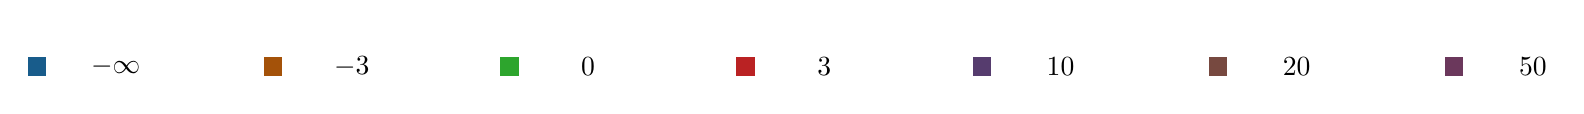
\begin{tikzpicture}
    %\centering
    %\draw[white,fill={rgb:red,31;green,119;blue,180}] (0,0) rectangle (2,1);
    \node[rectangle,fill={rgb:red,31;green,119;blue,180}] at (0,0) (1) {};
    \node[label] at (1,0) (2) {$-\infty$};
    \node[rectangle,fill={rgb:red,255;green,127;blue,14}] at (3,0) (3) {};
    \node[label] at (4,0) (4) {$-3$};
    \node[rectangle,fill={rgb:red,44;green,160;blue,44}] at (6,0) (5) {};
    \node[label] at (7,0) (6) {$0$};
    \node[rectangle,fill={rgb:red,214;green,39;blue,40}] at (9,0) (7) {};
    \node[label] at (10,0) (8) {$3$};
    \node[rectangle,fill={rgb:red,148;green,103;blue,189}] at (12,0) (9) {};
    \node[label] at (13,0) (10) {$10$};
    \node[rectangle,fill={rgb:red,140;green,86;blue,75}] at (15,0) (11) {};
    \node[label] at (16,0) (12) {$20$};
    \node[rectangle,fill={rgb:red,227;green,119;blue,194}] at (18,0) (13) {};
    %\node[rectangle,fill={rgb:red,255;green,0;blue,255}] at (18,0) (13) {};
    %\node[rectangle,fill={rgb:red,255;green,134;blue,218}] at (18,0) (13) {};
    \node[label] at (19,0) (14) {$50$};
\end{tikzpicture}
\end{minipage}
%\end{center}
\vspace{.5cm}
\begin{itemize}
    \item Comments:
    \begin{itemize}
        %\item When $\|\vct{x} - \vct{x}^{(0)}\|_{2}^{2}\geq 10 $ dB at initialization, we obtain a solution with high probability
        \item High probability to reach the true signal when the initial SNR is larger than $10$ dB.
        % \item $\text{SNR}(\vct{x},\vct{x}^{(0)})\geq 10 $ dB at initialization: Algorithm yields solution with high probability.
        %A solution can be reached with high probability when 
        %the initialization is within 10 dB SNR of the real solution
        %the algorithm is initialized within 10dB SNR of the solution
        %\item $\displaystyle \frac{\| |\mtx{\Phi} \vct{x}^{\ast} | - \vct{b} \|_2^2}{d^2} \leq 10^{-8}$ seems to be a good indicator of retrieval in the time-domain.
        %\item When $\displaystyle \frac{\left\lVert |\mtx{\Phi} \vct{x}^{\ast} | - \vct{b} \right\rVert_2^2}{d^2} \leq 10^{-8}$, 
        %a SNR greater than $20 \text{dB}$ is almost surely reached.
        \item $\displaystyle \frac{\left\lVert |\mtx{\Phi} \vct{x}^{\ast} | - \vct{b} \right\rVert^2}{d^2} \leq 10^{-8}$ implies almost surely that the output SNR is larger than $20$ dB. 
        \item Beyond $40\%$ of missing samples, the search space becomes very large: multiple solutions seem valid according to the first metric, whereas the output SNR remains low.
        %At high deleted fraction: Problem becomes under-constrained, slight increase of the probability of reaching $\vct{b}$ whereas SNR at convergence still decreases.
    \end{itemize}
\end{itemize}

    % \begin{algorithm}[H]
    % \caption{Compute attraction basin size}
    % \label{algoBassinAttraction}
    % \begin{algorithmic}
    % \REQUIRE{$S$ set of signal to noise ratios, $\hat{x}$ real solution, $\epsilon$ a success threshold
    % }
    % \ENSURE{$V$ set of signal to noise ratios where the algorithm converges}
    % \STATE $V \gets \{\}$
    % \FORALL{$\sigma \in S$}
    %     \STATE $n \sim \mathcal{N}_{\C}(0,\sigma)$
    %     \STATE $\xvbar^{(0)} \gets \hat{\xvbar} + n$
    %     \STATE $x_{pred} \gets Optimize(\xvbar^{(0)})$
    %     \IF{$\| |\Phi x_{pred}| - b \| < \epsilon$}
    %         \STATE{$V \gets V \cup \{\sigma\}$}
    %     \ENDIF
    % \ENDFOR
    % \RETURN $V$
    % \end{algorithmic}
    
    % \end{algorithm}

    % \begin{center}
    % \begin{minipage}{.3\linewidth}
    % \centering
    % \begin{tikzfigure}[Probability to reach $\frac{\| |\Phi x | - b \|_2^2}{\#\bar{v}^2} = 10^{-10}$]
    % \label{probaCVFourier}
    % \includegraphics[width=.8\linewidth,trim={0 0 0 15cm},clip]{figures/probaCVFourier-10.png}  
    % \end{tikzfigure}
    % \end{minipage}
    % \begin{minipage}{.3\linewidth}
    % \begin{tikzfigure}[Probability to reach $20 \text{DB SNR}$]
    % \label{probaCVTps}
    % \includegraphics[width=.8\linewidth,trim={0 0 0 15cm},clip]{figures/probaCVSNR.png}
    % \end{tikzfigure}
    % \end{minipage}
    % % \begin{minipage}{.3\linewidth}
    % % \blindtext[1]
    % % %The probability to reach $\frac{\| |\Phi x | - b \|_2^2}{\#\bar{v}^2} = 10^{-10}$ decreases rapidly as 
    % % \end{minipage}
    % \end{center}


%\vspace{.3cm}
% TODO suppr Cadre et passer dans ongoing work
% \innerblock{Initialization strategies}{
% %Several initialization strategies have been tested and compared:
% %New initialization by adaptation of Spectral Method~\cite{Candes2015b}: 
% For the phase retrieval problem, the Spectral initialization is~\cite{Candes2015b}:
% \begin{align}
% \label{eqn:spectralInit}
% \mtx{Y} &=\frac {1}{L}\sum _{r=1}^{L}b_{r} \mtx{\Phi}_{r} \mtx{\Phi}_{r}^{\mathsf{H}}\\
% \vct{x}^{(0)} &\gets \text{GEV}(\mtx{Y})
% \end{align}
% GEV: Eigenvector with the greatest eigenvalue.

% We rewrite the audio inpainting problem as:
% \begin{equation}
%     \begin{bmatrix}
%     \vct{x}_{\bar{v}} \\ \cdot 
%     \end{bmatrix} =
%     \underset{\widetilde{\vct{x}}_{d + 1} = 1, \; \widetilde{\vct{x}} \in \R^{d+1}}{\text{argmin}}\,\|  |\widetilde{\mtx{\Phi}} \widetilde{\vct{x}} | -\vct{b}\|^{2},
% \end{equation}
% where $\widetilde{\Phi} = \begin{bmatrix} 
%         \Phi_{\overline{v}} & \Phi_v x_v\\
%     \end{bmatrix} \in \mathbb{C}^{L \times (d+1)}$

% \begin{align*}
%     \widetilde{\vct{x}}^{(0)} &\gets \text{SPECTRALMETHOD}(\widetilde{\mtx{\Phi}}) \\
%     \vct{x}_{\bar{v}}^{(0)} &\gets \mtx{\Phi}_{\bar{v}}^{\mathsf{H}} \left( \mtx{\Phi}_{\overline{v}} \widetilde{\vct{x}}_{:d} + (\widetilde{\vct{x}}_{d+1} -1 ) \Phi_v x_v \right)
% \end{align*}

%\vct{x}_{\bar{v}}^{\ast} =  \underset{\vct{x}_{v}= \vct{y}, \; \vct{x} \in \R^{L}}{\text{argmin}}\,\|  |\mtx{\Phi}_v \vct{x}_v + \mtx{\Phi}_{\bar{v}} \vct{x}_{\bar{v}} | -\vct{b}\|^{2}
% \begin{itemize}
%     \item Strategies
% \begin{itemize}
%     \item $\xvbar \gets 0$
%     \item $\xvbar \sim \mathcal{N}(0,1)$
%     \item Spectral Method \cite{Candes2015b}\\
%     \begin{align}
%     %\label{eqn:reformulationWirtinger}
%     \vct{x}_{\bar{v}}^{\ast} &=  \underset{\vct{x}_{v}= \vct{y}, \; \vct{x} \in \R^{L}}{\text{argmin}}\,\|  |\mtx{\Phi}_v \vct{x}_v + \mtx{\Phi}_{\bar{v}} \vct{x}_{\bar{v}} | -\vct{b}\|^{2} \\
% &=  \underset{\widetilde{\vct{x}}_{d + 1} = 1, \; \widetilde{\vct{x}} \in \R^{d+1}}{\text{argmin}}\,\|  |\widetilde{\mtx{\Phi}} \widetilde{\vct{x}} | -\vct{b}\|^{2},
% \end{align}
% where $\widetilde{\Phi} = \begin{bmatrix} 
%         \Phi_{\overline{v}} & \Phi_v x_v\\
%     \end{bmatrix} \in \mathcal{M}_{L \times d+1}$, and $d=\#\bar{v}$
% By relaxing the constraint $\widetilde{\vct{x}}_{d + 1} = 1$, The problem can be reformulated as a Phase retrieval problem, which can be initialized by the spectral method \cite{Candes2015b}. Then, the first $d$ coordinates of $\widetilde{x}$ are used to initialize $\xvbar$
% \end{itemize}
% \item Results
% Initializing the unknown signal to zero
% No significant difference between the strategies has been found. 
% \end{itemize}
% }
% \vspace{-1.8cm}
%\vspace{-2cm}
}

\block{ONGOING WORK}{
\begin{itemize}
    \item Theoretical study on the \textbf{uniqueness} and the \textbf{stability of the solution}.
    \item \textbf{Initialization strategy} by adapting the \textbf{spectral method}~\cite{Candes2015b}:
    \begin{itemize}
        \item Rewrite the problem as:
        \begin{equation*}
        \begin{bmatrix}
        \vct{x}_{\bar{v}}^{\ast} \\ \cdot 
        \end{bmatrix} =
        %\underset{\widetilde{\vct{x}}_{d + 1} = 1, \; \widetilde{\vct{x}} \in \R^{d+1}}{\text{argmin}}\,\|  |\widetilde{\mtx{\Phi}} \widetilde{\vct{x}} | -\vct{b}\|^{2}
        \underset{\widetilde{\vct{x}}_{\overline{v}} \in \R^{d}}{\text{argmin}}\, \left\lVert  |\widetilde{\mtx{\Phi}} \begin{bmatrix}
        \vct{x}_{\bar{v}} \\ 1 
        \end{bmatrix}| -\vct{b}\right\rVert^{2} \quad \text{with} \quad \widetilde{\mtx{\Phi}} = [\mtx{\Phi_{\overline{v}} }
        ;\mtx{\Phi}_v \vct{x}_v] \in \mathbb{C}^{L \times (d+1)}
       % \quad \text{s.t.} \quad \widetilde{\vct{x}}_}{v}(d + 1) = 1
        \end{equation*}
  \item Let $\widetilde{\vct{x}} = \begin{bmatrix}
        \vct{x}_{\bar{v}} \\ 1 
        \end{bmatrix}$.
        The above problem is equivalent to:
  \begin{equation*}
       \widetilde{\vct{x}}^{\ast}=
        \underset{\widetilde{\vct{x}} \in \R^{d+1}}{\text{argmin}}\,\left\lVert |\widetilde{\mtx{\Phi}} \widetilde{\vct{x}} | -\vct{b}\right\rVert^{2} 
        \quad \text{s.t.} \quad \widetilde{\vct{x}}_{d + 1} = 1
        \end{equation*}
       \item Without constraint, this problem boils down to phase retrieval $\to$ initialization with the spectral method:
       \begin{equation*}
       \widetilde{\vct{x}}^{\text{sp}} \gets \text{GEV}\left(\frac {1}{L}\sum _{k=1}^{L}b_{k} \vct{e}_k^{\mathsf{H}} \widetilde{\mtx{\Phi}}  \widetilde{\mtx{\Phi}}^{\mathsf{H}} \vct{e}_k \right)
       \end{equation*}
       (GEV: Eigenvector with the highest eigenvalue)
       \item Considering the constraint, we seek the following initialization: 
        % \begin{align*}
        % \widetilde{\vct{x}}^{(0)} = \underset{\widetilde{\vct{x}} \in \R^{d+1}}{\text{argmin}}\, \left\lVert \widetilde{\vct{x}}_{d+1} - 1\right\rVert^{2} 
        % \quad \text{s.t.} \quad
        % \widetilde{\mtx{\Phi}}\widetilde{\vct{x}}=\mtx{\Phi}_v \vct{x}_v + \mtx{\Phi}_{\bar{v}} \widetilde{\vct{x}}_{:d}
        % \end{align*}
        \begin{equation*}
            \vct{x}_{\bar{v}}^{(0)} = \underset{\vct{x}_{\bar{v}} \in \R^{d}}{\text{argmin}}\left\lVert \widetilde{\mtx{\Phi}}\widetilde{\vct{x}}^{\text{sp}}
            - \left(\mtx{\Phi}_v \vct{x}_v + \mtx{\Phi}_{\bar{v}} \vct{x}_{\bar{v}} \right) \right\rVert^{2}
        \end{equation*}
        which yields:
        \begin{equation*}
            \vct{x}_{\bar{v}}^{(0)} = \mtx{\Phi}_{\bar{v}}^{\mathsf{H}} \left( \mtx{\Phi}_{\overline{v}} \widetilde{\vct{x}}_{:d}^{\text{sp}} + (\widetilde{\vct{x}}_{d+1}^{\text{sp}} -1 ) \Phi_v x_v \right)
        \end{equation*}
\end{itemize}

     %\item Rewrite our problem with $\widetilde{\mtx{\Phi}}$:
     
     
       % \item Powerful initialization of the phase retrieval problem proposed by ~\cite{Candes2015b}: 
        
        %\begin{align*}
        %\label{eqn:spectralInit}
        %\mtx{Y} &=\frac {1}{L}\sum _{k=1}^{L}b_{k} \vct{e}_k \mtx{\Phi} \mtx{\Phi}^{\mathsf{H}} \vct{e}_k\\
        %\vct{x}^{(0)} &\gets \text{GEV}(\mtx{Y})
        %\end{align*}
        %GEV: Eigenvector with the greatest eigenvalue.
       
        %\begin{equation*}
        %\begin{bmatrix}
        %\vct{x}_{\bar{v}}^{\ast} \\ \cdot 
        %\end{bmatrix} =
        %\underset{\widetilde{\vct{x}}_{d + 1} = 1, \; \widetilde{\vct{x}} \in \R^{d+1}}{\text{argmin}}\,\|  |\widetilde{\mtx{\Phi}} \widetilde{\vct{x}} | -\vct{b}\|^{2}
        %\underset{\widetilde{\vct{x}} \in \R^{d+1}}{\text{argmin}}\,\|  |\widetilde{\mtx{\Phi}} \widetilde{\vct{x}} | -\vct{b}\|^{2} 
        %\quad \text{s.t.} \quad \widetilde{\vct{x}}_{d + 1} = 1
        %,
        %\end{equation*}
        %where $\widetilde{\Phi} = \begin{bmatrix} 
       % \Phi_{\overline{v}} & \Phi_v x_v\\
        %\end{bmatrix} \in \mathbb{C}^{L \times (d+1)}$.
        % \item Delete the constraint $\widetilde{\vct{x}}_{d + 1} = 1$ and use the spectral method with $\widetilde{\mtx{\Phi}}$ as observation matrix to compute $\widetilde{\vct{x}}^{(0)}$.
        % \item Reintroduce the constraint using the last coordinate of $\widetilde{\vct{x}}^{(0)}$
        % \begin{equation*}
        %     \vct{x}_{\bar{v}}^{(0)} \gets \mtx{\Phi}_{\bar{v}}^{\mathsf{H}} \left( \mtx{\Phi}_{\overline{v}} \widetilde{\vct{x}}_{:d}^{(0)} + (\widetilde{\vct{x}}_{d+1}^{(0)} -1 ) \Phi_v x_v \right)
        % \end{equation*}
        % \item Possibility of a theoretical guaranty.
    
    %\item Theoretical study of the stability of a solution. 
    \item \textbf{Lifting-based methods}~\cite{Candes2011} to find $\vct{u}$
    %\begin{itemize}
        %\item Relaxing the constraint $\vct{u} = phase(\mtx{\Phi} \vct{x})$ by $|\vct{u}|=1$
        %\item Obtain the following lifted formulation:
        \begin{align*}
            \underset{\mtx{\widetilde{U}} \succeq 0}{\text{min}} \;
            {\text{trace}(\mtx{C}\mtx{\widetilde{U}})} \quad 
             \text{s.t} \;  \diag(\mtx{\widetilde{U}})=1,
            \end{align*}
            where $\mtx{C} = \mtx{A^{\mathsf{H}}}\mtx{A}$  with  $\mtx{A} =[\mtx{\Phi}_{\bar{v}}^{\mathsf{H}}\diag(\vct{b}), -\vct{x}_{v}]$ and $\mtx{\widetilde{U}} = \vct{\Tilde{u}}^{\mathsf{H}}\vct{\Tilde{u}}, \vct{\Tilde{u}} = [\vct{u},1]^{\mathsf{T}}$
    %\end{itemize}
       %\item Relax the constraint of \eqref{eqn:phaseprob2} and solve it using semidefinite optimization methods 
    \item Extension to \textbf{noisy observations} i.e.  $|\mtx{\Phi} \vct{x} | = \vct{b} + \eta$ where $\eta$ is some noise. 
\end{itemize}
% \vspace{-1.8cm}
\vspace{-2cm}
}
\end{columns}

\begin{columns}
\column{1}
\block{REFERENCES}{
 \printbibliography[heading=none]
}
\end{columns}

\end{document}